\documentclass{scrartcl}[a4paper, 11pt]
\usepackage{graphicx} % Required for inserting images
\usepackage{hyperref}
\usepackage{fullpage}
\usepackage{csquotes}
\usepackage{geometry}
\usepackage{float}

\geometry{a4paper, top=15mm, bottom=25mm, left=20mm, right=20mm}
\hypersetup{
    colorlinks=true,     
    urlcolor=blue,
    }

\subject{184.702 - Machine Learning}
\title{Exercise 0 - Dataset description}
\author{Florian Engl (12102619),\\ Lukas Sichert (12114770),\\ Kristof Dadic (12105475)}
\date{October 2024}

\setlength{\parindent}{0mm}

\begin{document}

\maketitle

\section{Census Income \href{https://archive.ics.uci.edu/dataset/2/adult}{Dataset}}
    The Census Income Dataset is data used to predict whether a person has an annual salary of over or under 50 thousand dollars and also helps to predict which attributes have a greater influence on income. The United States census is taken by the United States Census Bureau every two years and this particular dataset was taken from the 1994 census.
    \vspace{4mm}
    
    It has 14+1 attributes the last one being the target \enquote{income} and 48~842 instances. The attributes are:

    \begin{itemize}
        \item \underline{age:} is a ratio attribute with integer values in [17,90].
        \item \underline{workclass:} is a nominal attribute with the values: \textit{\enquote{Private}, \enquote{Self-emp-not-inc}, \enquote{Self-emp-inc}, \enquote{Federal-gov}, \enquote{Local-gov}, \enquote{State-gov}, \enquote{Without-pay}, \enquote{Never-worked}}.
        \item \underline{fnlwgt:} is a ratio attribute and quantifies how many people the census bureau believes the observation represents. The abbreviation stands for final weight and takes integer values between 12~285 and 1~490~400. 
        \item \underline{education:} is a nominal attribute too with the ordinal values: \textit{\enquote{Preschool}, \enquote{1\textsuperscript{st}-4\textsuperscript{th}}, \enquote{5\textsuperscript{th}- 6\textsuperscript{th}}, 
        \enquote{7\textsuperscript{th}-8\textsuperscript{th}}, \enquote{9\textsuperscript{th}}, \enquote{10\textsuperscript{th}}, \enquote{11\textsuperscript{th}}, 
        \enquote{12\textsuperscript{th}}}, \textit{\enquote{HS-Grad}}, \textit{\enquote{Some-college}}, 
        \textit{\enquote{Assoc-voc}}, \textit{\enquote{Assoc-acdm}},\textit{\enquote{Bachelors}},
        \textit{\enquote{Masters}}, \textit{\enquote{Prof-school}} and \textit{\enquote{Doctorate}}.
        \item \underline{education-nom:} is an integer value in $[1,16]$ which is an alternative description for the degree of education. Here 1 represents the lowest education \textit{\enquote{Prescool}} and 16 the highest \textit{\enquote{Doctorate}}. This column is not necessary as all information is also in the \underline{education} column, but it is helpful for data-preprocessing.
        \item \underline{marital-status:} this nominal attribute can take the values: 
        \textit{\enquote{Married-civ-spouse}}, \textit{\enquote{Divorced}}, \textit{\enquote{Never-married}}, \textit{\enquote{Seperated}}, \textit{\enquote{Widowed}}, \textit{\enquote{Married-spouse-absend}}, \textit{\enquote{Married-AF-spouse}}. \linebreak Here \textit{\enquote{civ}} means civilian and 
        \textit{\enquote{AF}} means Armed-Forces.
        \item \underline{occupation:} is a nominal attribute, which groups the occupation into the following classes 
        \textit{\enquote{Adm-clerical}}, \textit{\enquote{Armed-Forces}}, \textit{\enquote{Craft-repair}},
        \textit{\enquote{Exec-managerial}}, \textit{\enquote{Farming-fishing}}, \textit{\enquote{Handlers-cleaners}},
        \textit{\enquote{Other}}, \textit{\enquote{Priv-house-serv}}, \textit{\enquote{Prof-specialty}}, \textit{\enquote{Protective-Serv}}, \textit{\enquote{Sales}}, \linebreak \textit{\enquote{Tech-Support}}.
        \item \underline{relationship:} represents the family-relationship and can take the values \textit{\enquote{Wife}}, \textit{\enquote{Own-child}},  \textit{\enquote{Husband}}, \textit{\enquote{Not-in-family}}, \textit{\enquote{Other-relative}} and \textit{\enquote{Unmarried}}. It is therefore also a nominal attribute.
        \item \underline{race:} is another nominal attribute with the values  \textit{\enquote{White}},  \textit{\enquote{Asian-Pac-Islander}},  \textit{\enquote{Amer-Indian-Eskimo}},  \textit{\enquote{Black}} and  \textit{\enquote{Other}}.
        \item \underline{sex:} is a nominal attribute with the two values  \textit{\enquote{male}} and  \textit{\enquote{female}}.
        \item \underline{capital-gain:} is a ratio attribute with integer values in [0,99999]. 
        \item \underline{capital-loss:} is also a ratio quantity with values between 0 and 2356.
        \item \underline{hours-per-week:} is a ratio attribute with integer values in [1,99].
        \item \underline{native-country:} is a nominal attribute with the levels 
        \enquote{\textit{United-States}}, \enquote{\textit{Cambodia}}, \enquote{\textit{England}}, \enquote{\textit{Puerto-Rico}}, \enquote{\textit{Canada}}, \enquote{\textit{Germany}}, \enquote{\textit{Outlying-US (Guam-USVI-etc)}}, \enquote{\textit{India}}, \enquote{\textit{Japan}}, \enquote{\textit{Greece}}, \enquote{\textit{South}}, \enquote{\textit{China}}, \enquote{\textit{Cuba}}, \enquote{\textit{Iran}}, \enquote{\textit{Honduras}}, \enquote{\textit{Philippines}}, \enquote{\textit{Italy}}, \enquote{\textit{Poland}}, \enquote{\textit{Jamaica}}, \enquote{\textit{Vietnam}}, \enquote{\textit{Mexico}}, \enquote{\textit{Portugal}}, \enquote{\textit{Ireland}}, \enquote{\textit{France}}, \enquote{\textit{Dominican-Republic}}, \enquote{\textit{Laos}}, \enquote{\textit{Ecuador}}, \enquote{\textit{Taiwan}}, \enquote{\textit{Haiti}}, \enquote{\textit{Columbia}}, \enquote{\textit{Hungary}}, \enquote{\textit{Guatemala}}, \enquote{\textit{Nicaragua}}, \enquote{\textit{Scotland}}, \enquote{\textit{Thailand}}, \enquote{\textit{Yugoslavia}}, \enquote{\textit{El-Salvador}}, \enquote{\textit{Trinidad\&Tobago}}, \enquote{\textit{Peru}}, \linebreak \enquote{\textit{Hong Kong}}, \enquote{\textit{Netherlands}}.
        \item \underline{income:} is the target attribute. It can take the values 
        \enquote{$>$4\textit{50K}} and \enquote{\textit{$\leq$50K}}. In this dataset the distribution of these values is 
        $$
            \leq 50K : 76 \% \quad >50K: 23\%.
        $$

    \end{itemize}
    The columns \textit{workclass, occupation} and \textit{native-country} have missing values, which needs to be addressed during the preprocessing-step.
    Also, as the numerical values have different ranges, we will need to scale them appropriately in the preprocessing-step.
    
    Because the target attribute can only take two discrete values the dataset is suited classification.

    \begin{figure}[H]
        \centering
        \begin{minipage}[b]{0.45\linewidth}
            \centering
            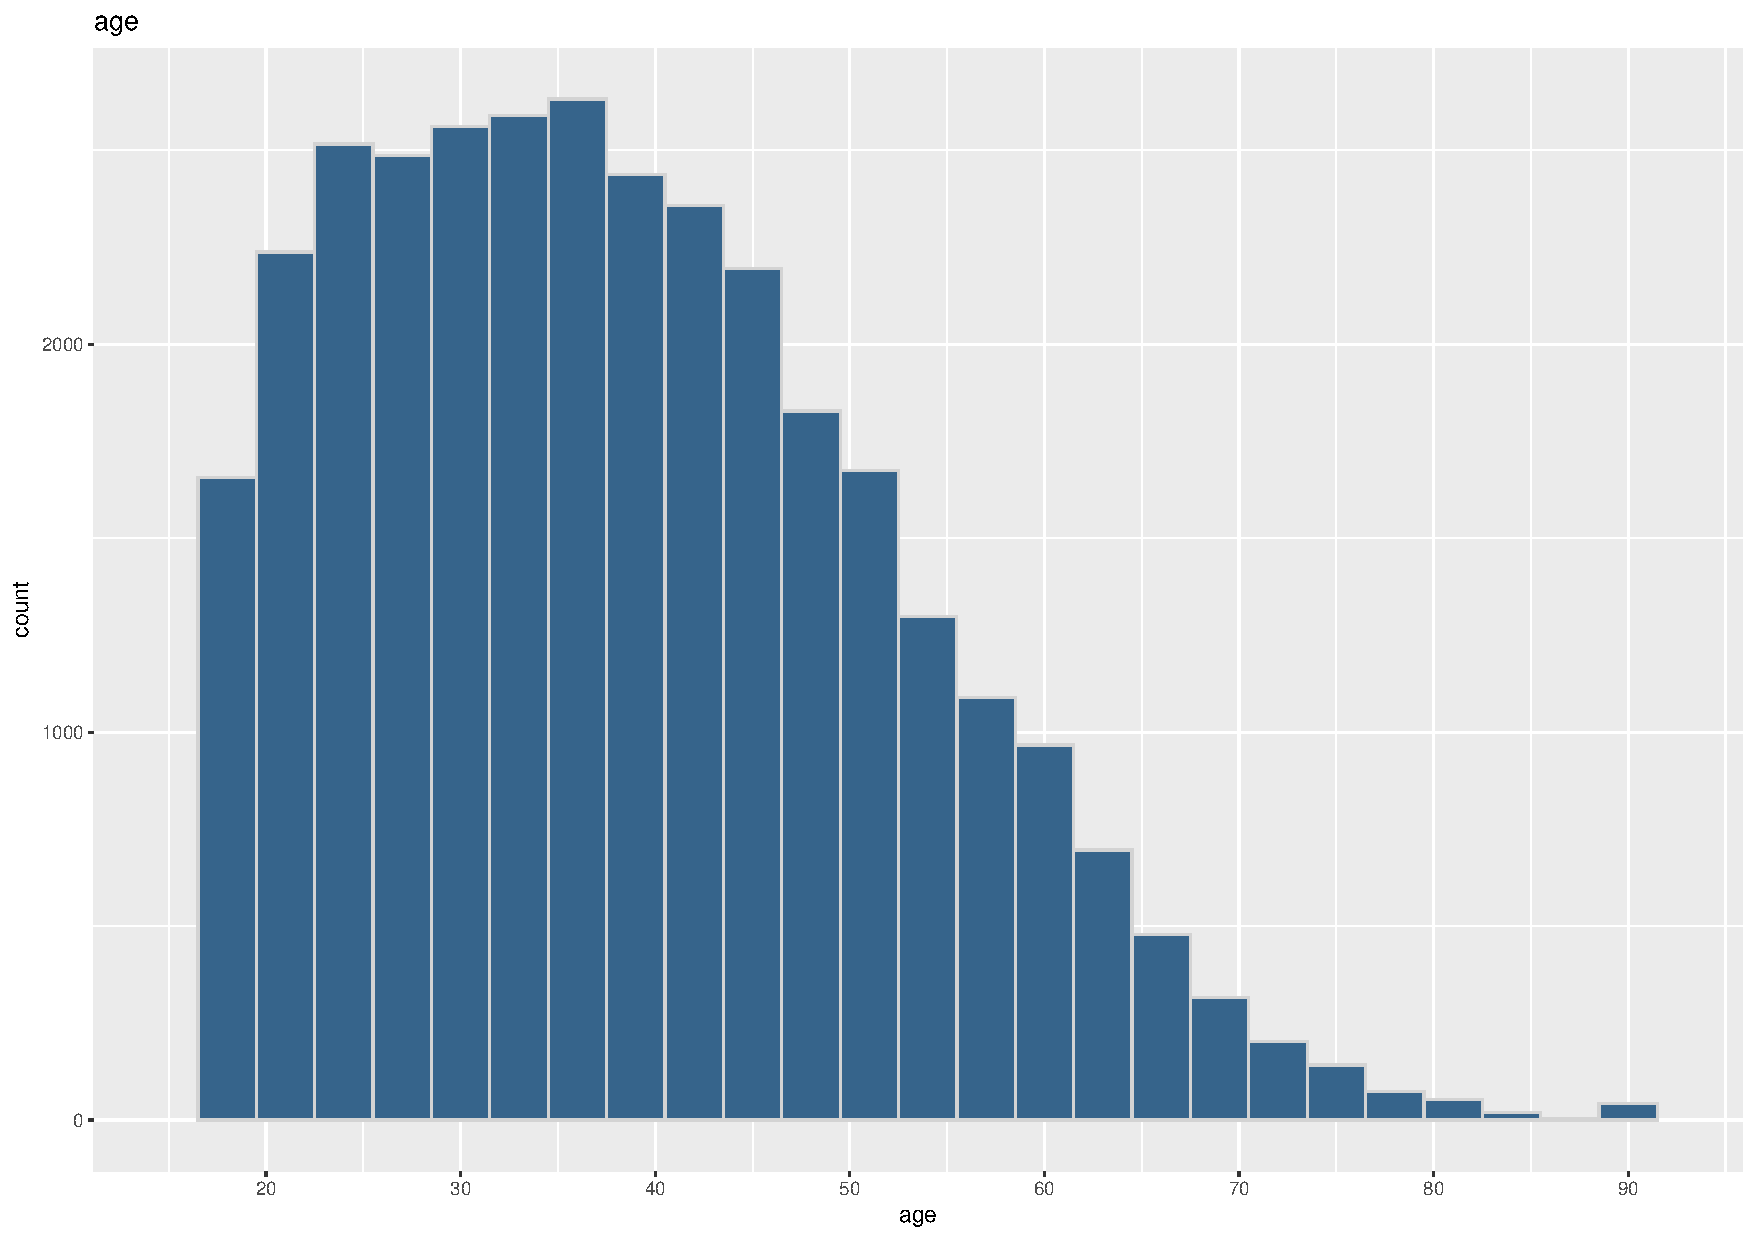
\includegraphics[width=\textwidth]{figures/age.pdf} 
        \end{minipage} 
        \begin{minipage}[b]{0.45\linewidth}
            \centering
            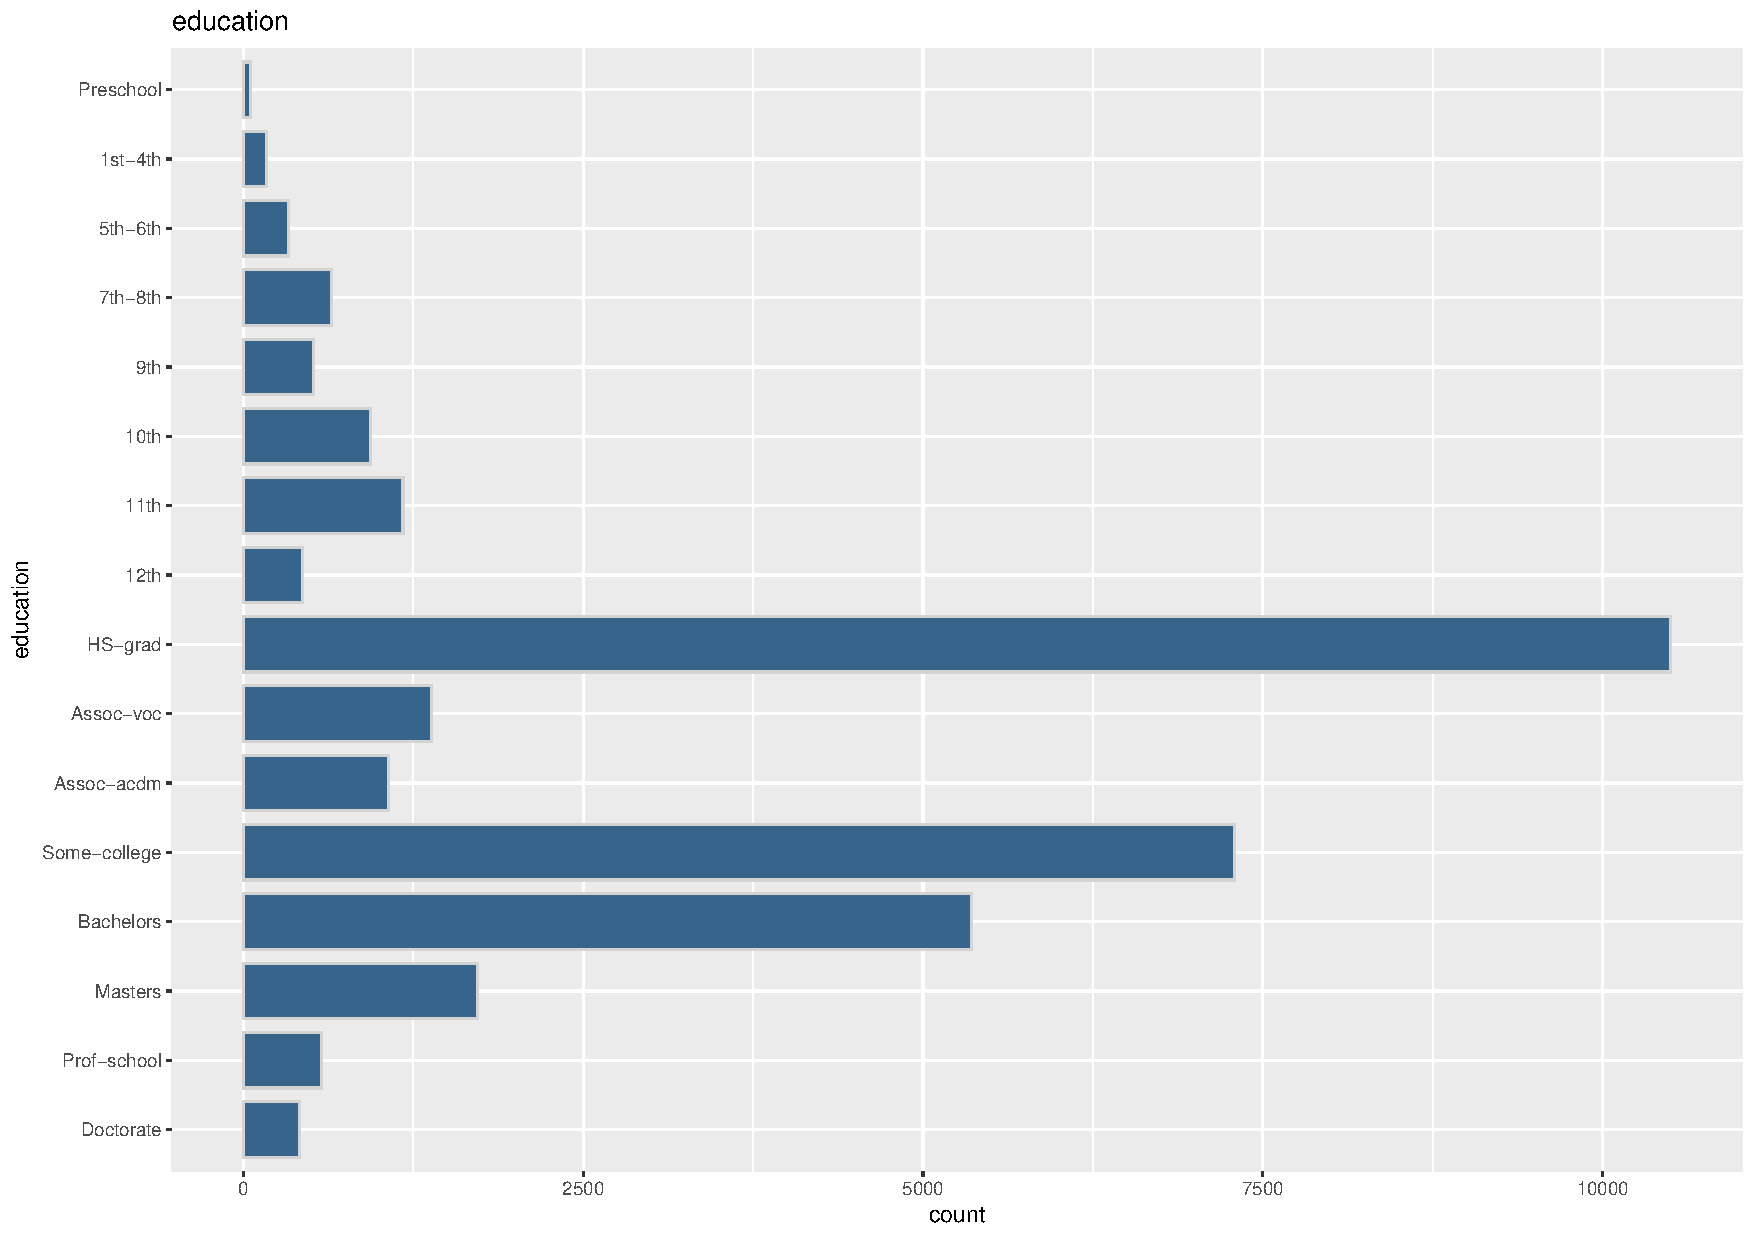
\includegraphics[width=\textwidth]{figures/education.pdf} 
        \end{minipage} 
        \begin{minipage}[b]{0.45\linewidth}
            \centering
            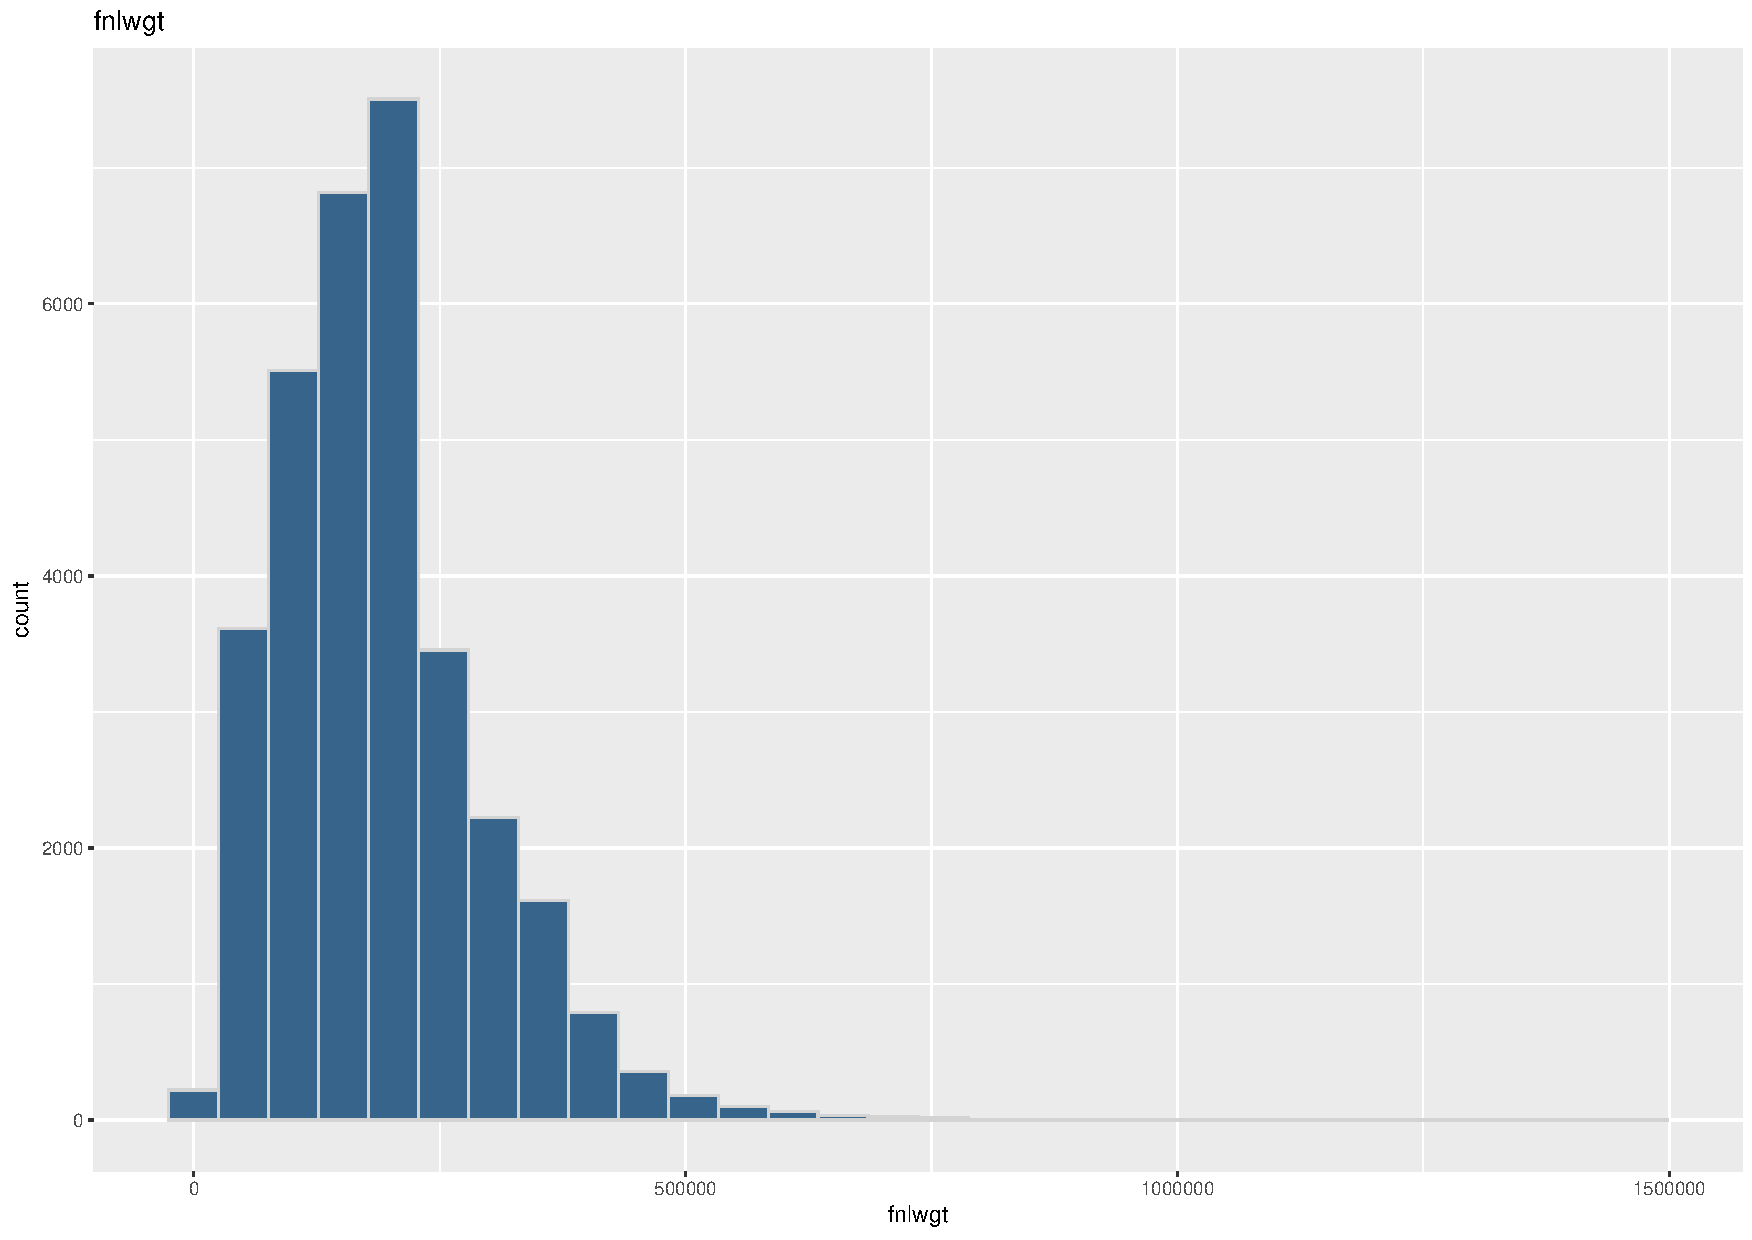
\includegraphics[width=\textwidth]{figures/fnlwgt.pdf} 
        \end{minipage}
        \begin{minipage}[b]{0.45\linewidth}
            \centering
            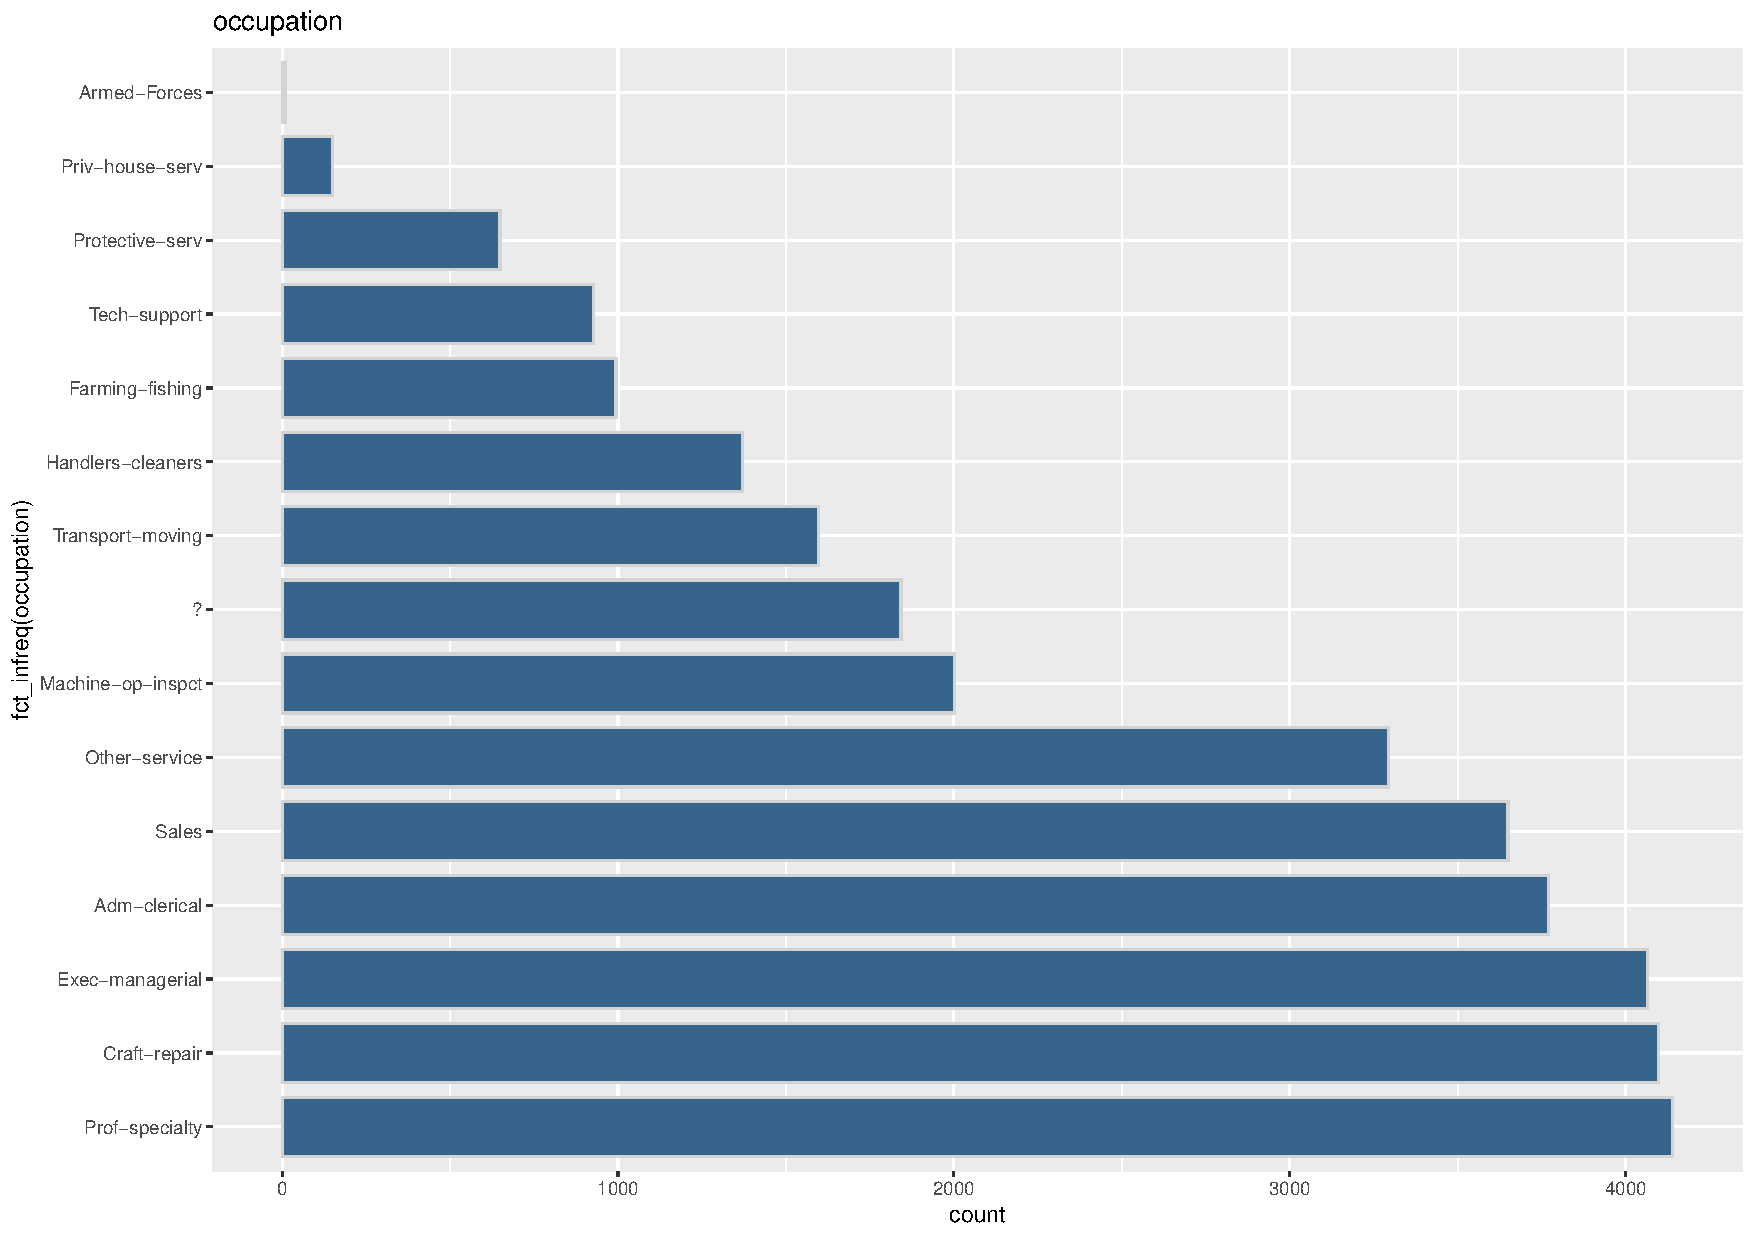
\includegraphics[width=\textwidth]{figures/occupation.pdf} 
        \end{minipage} 
    \end{figure}
    
\section{Superconductivity \href{https://archive.ics.uci.edu/dataset/464/superconductivty+data}{Dataset}}

Superconductors are of growing importance for different uses, ranging from nuclear fusion to modern types of transportation. A major problem with the use of superconductors has always been the fact that they need to be cooled below the critical temperature for the resistance to drop dramatically. Therefore it has been an interest of modern science to make superconductors with ever higher critical temperatures. We chose this topic as one of us is studying physics and is therefore interested in superconductors and because we think they will play an important role in the technological future.
\vspace{4mm}

The chosen dataset contains the chemical data for different superconductors with the corresponding critical temperature. There is a second file that contains the specific chemical formula and the critical temperature. It has 81+1 attributes the last one being the target attribute, the critical temperature, and 21~263 instances. There are no missing values and all attributes (except for the chemical formula in the second file) are numerical. The attributes are:


\begin{itemize}
    \item \underline{number\_of\_elements:} An integer value describing the number of elements used in the alloy.
    \item \underline{atomic\_mass:} Here the mean, weighted mean, geometric mean, entropy, weighted entropy, range, weighted range, standard deviation and weighted standard deviation are the distinct attributes of this quantity. They are all continuous variables. 
    \item \underline{fie:} The attributes have the same structure as above.
    \item \underline{atomic\_radius:} The attributes have the same structure as above except for the range, which is an integer.
    \item \underline{Density:} The attributes have the same structure as above.
    \item \underline{ElectronAffinity:} The attributes have the same structure as above.
    \item \underline{FusionHeat:} The attributes have the same structure as above.
    \item \underline{ThermalConductivity:} The attributes have the same structure as above.
    \item \underline{Valence:} The attributes have the same structure as above except for the range, which is an integer.
    \item \underline{critical\_temp:} This is the target variable. It ranges from $0.00021$ to $185$ with a mean of $34.42$ and standard deviation of $34.25$.
\end{itemize}

In the figure below the attributes' standard deviations are plotted against their index. Clearly, there are a few attributes with a very high standard deviation that will likely need rescaling. Upon further investigation, we identified these attributes as the mean, weighted mean, geometric mean, range, weighted range, standard deviation and weighted standard deviation of \textit{Density}, likely due to the choice of unit.

Because the target attribute is continuous the dataset is suited for regression.

\begin{figure}[H]
    \centering
    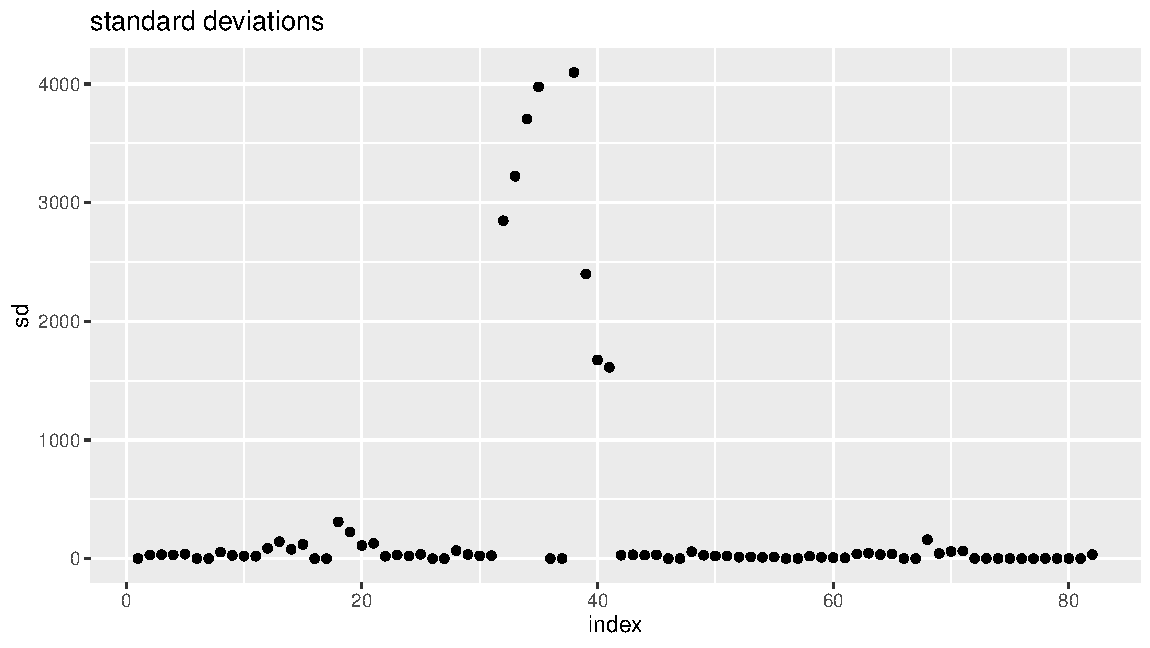
\includegraphics[width=0.8\linewidth]{figures/sd.pdf}
\end{figure}


\end{document}
